% ===============================================================================================
% ===============================================================================================
% =====================================Conference Logistics======================================
% ===============================================================================================
% ===============================================================================================

\section{Conference Logistics}

\subsection{Date Selection}


We propose the conference be held on either of the following dates: 
\begin{enumerate}
	\item Thursday, April 8$^{th}$ - Sunday, April 11$^{th}$ 
	\item Thursday, April 15$^{th}$ - Sunday, April 18$^{th}$
\end{enumerate}
We believe either of these dates would serve as an appropriate first choice because they avoid major conflict dates like finals and spring break for most schools. Additionally, mid-April offers pleasant, mild, weather in Champaign. The reason for proposing two weekends to host the conference is due to the UIUC tradition of hosting Mom's Weekend on or near the first weekend in April. The Illinois Mom's Association has not yet announced their 2021 dates but, to avoid potential conflict, we suggest two dates. In the event that both of these dates are unavailable our backup date is 
\begin{itemize}
	\item Thursday, April 1$^{st}$ - Sunday, April 4$^{th}$.  
\end{itemize}
This is a backup date because Easter falls on that Sunday. In general, this 
should be avoided. In this case we found that holding the conference at the end 
of April would conflict with finals for students and holding it earlier in 
March would conflict with several spring breaks as well as having potentially 
poorer weather. \textbf{A detailed graphical conflict schedule can be found in Appendix 
\ref{appendix:schedule} on page \pageref{appendix:schedule}.} 

\subsection{Conference Facilities}

\textbf{The Illini Union}\\

\begin{figure}[H]
	\centering
	\begin{subfigure}{0.5\textwidth}
		\centering
		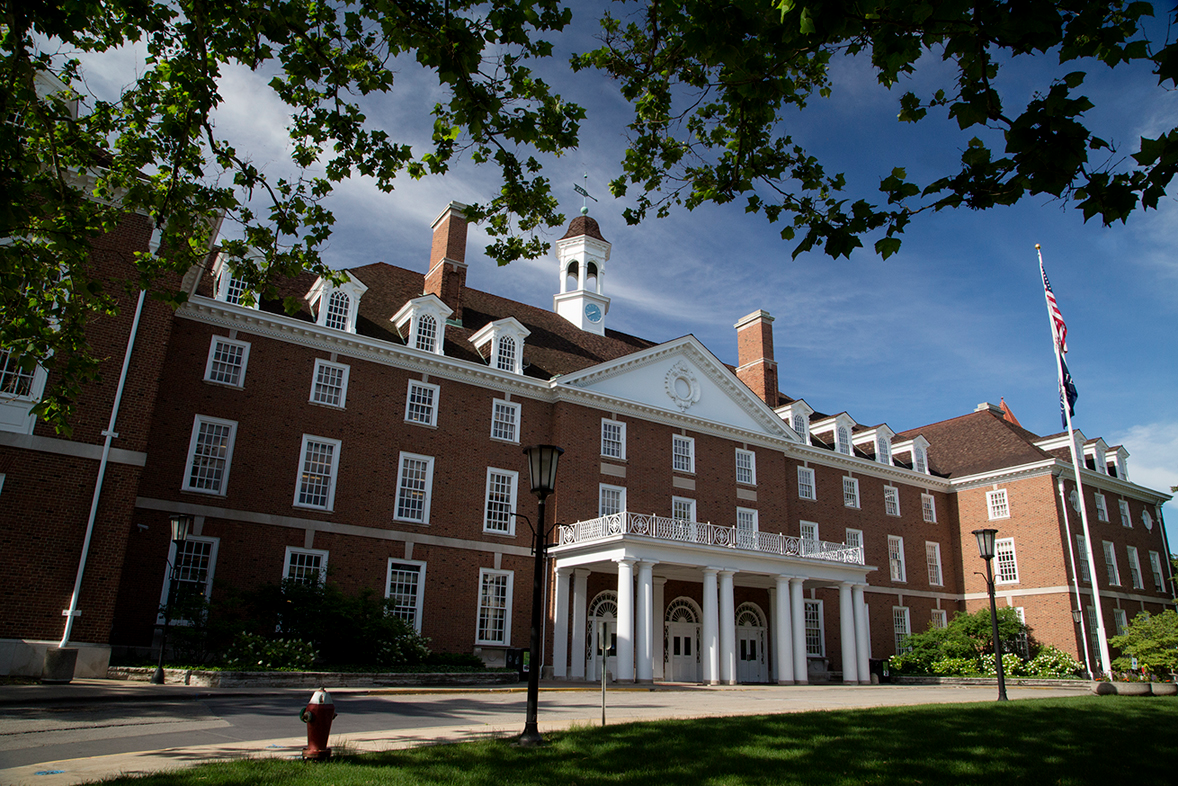
\includegraphics[scale=0.2]{illini-union.png}
	\end{subfigure}%
	\begin{subfigure}{0.5\textwidth}
		\centering
		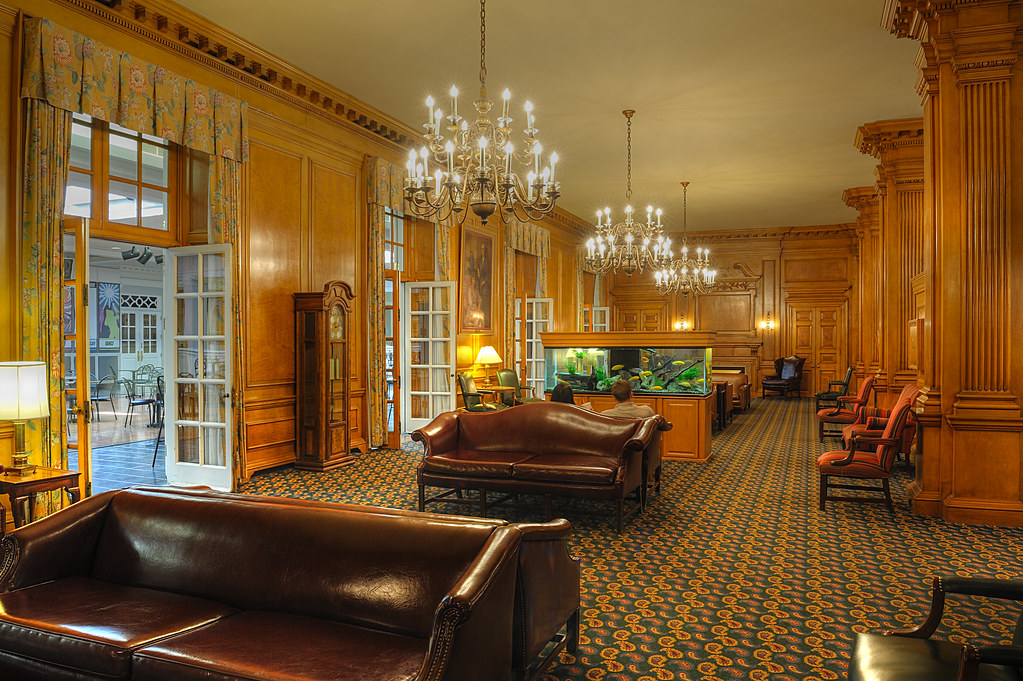
\includegraphics[width=0.9\linewidth]{union-inside.jpg}
	\end{subfigure}
	\caption{Illini Student Union}		
\end{figure} 


The Illini Union is capable of hosting the entire technical program of the ANS 
Student Conference. This keeps the conference contained in one convenient 
location while being within easy access of the rest of the campus. Technical 
sessions will be held in a combination of rooms on the second, third, and 
fourth floors of The Union. Each of these rooms have at least enough capacity 
for 42 people, lecture style, and A/V capability. There will also be rooms 
available to have panels and workshops during the course of the technical 
program. The Illini Rooms A and B will be a combined space for the career fair 
while Illini Room C and the south lounge will host the poster sessions. We will 
keep the space open to allow the poster sessions and career fair to share 
attendance and encourage networking. A detailed list of room capacities and 
floor plans are located in Appendix \ref{appendix:building}: Building Layout on 
page \pageref{appendix:building}. \\


\subsection{Banquet Space}
\subsubsection{Garden Hotel in Urbana}
The opening ceremony dinner on Thursday night will be hosted at the Garden Hotel in Urbana. It has a seating capacity of 600 people in round tables, offers in-house catering, and AV capabilities. This location was chosen for its convenience, as it would be the primary hotel for the conference. 

\begin{figure}[H]
    \centering
    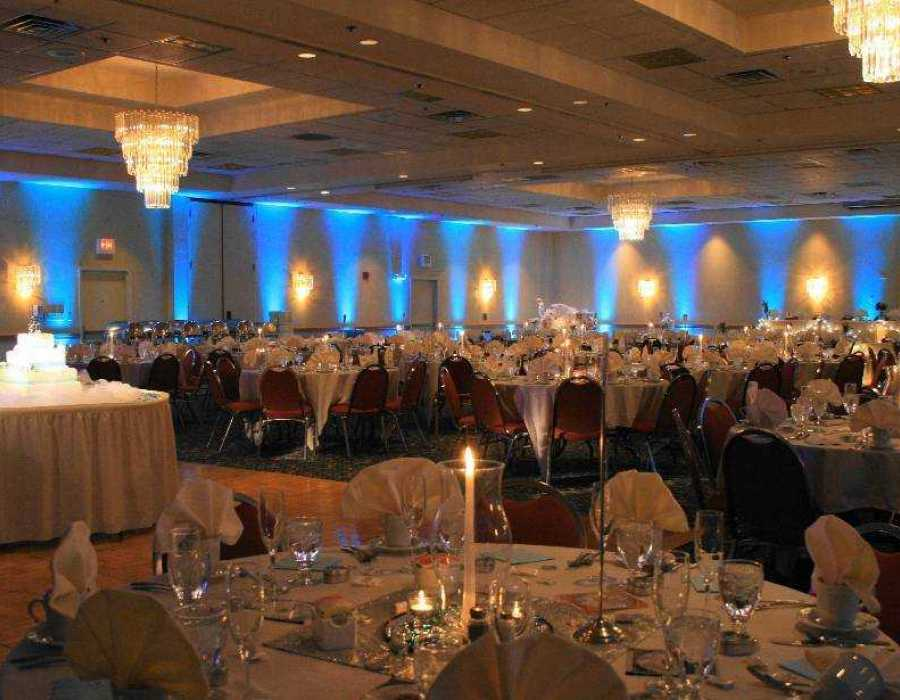
\includegraphics[width=0.5\textwidth]{garden_dinner.jpg}
    \caption{The Garden Hotel Banquet Hall with capacity for 600 people in round tables.}
\end{figure}

\subsubsection{I Hotel}
Dinner on Friday night will be hosted at the I Hotel. The I Hotel is undergoing an expansion that will increase the capacity of their banquet space to 690 people in round tables. Catering is provided by University Catering which avoids a 20\% gratuity charge because of its association with the University of Illinois. This expansion is set to be completed by Fall 2020. We will be hosting a social at the 77 Club in Memorial Stadium, just up the street. Information about the I Hotel expansion is included in Appendix D.

\begin{figure}[H]
    \centering
    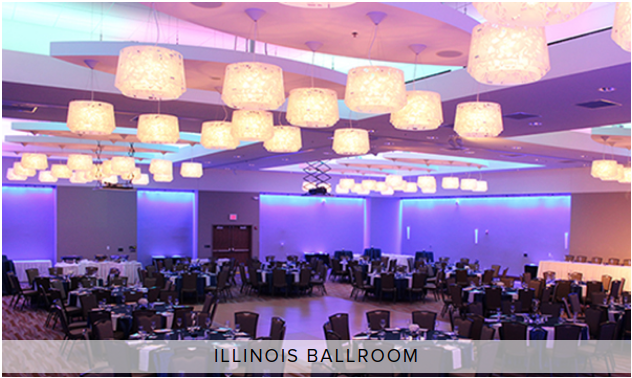
\includegraphics[width=0.75\textwidth]{ihotel-dinner.png}
    \caption{The current 400-person banquet space at the IHotel is pictured 
        above. A new, 690-person ballroom will be available in 2020.}
\end{figure}

\subsubsection{Illini Union}
After the career fair is taken down on Saturday, the final dinner will be set up in the combined Illini Rooms, which has a seating capacity of 496 people in round tables. Catering will be provided by University Catering which allows us to avoid the 20\% gratuity for services. A floorplan for the Illini Rooms in round tables is available in Appendix D.\\

\begin{figure}[H]
    \centering
    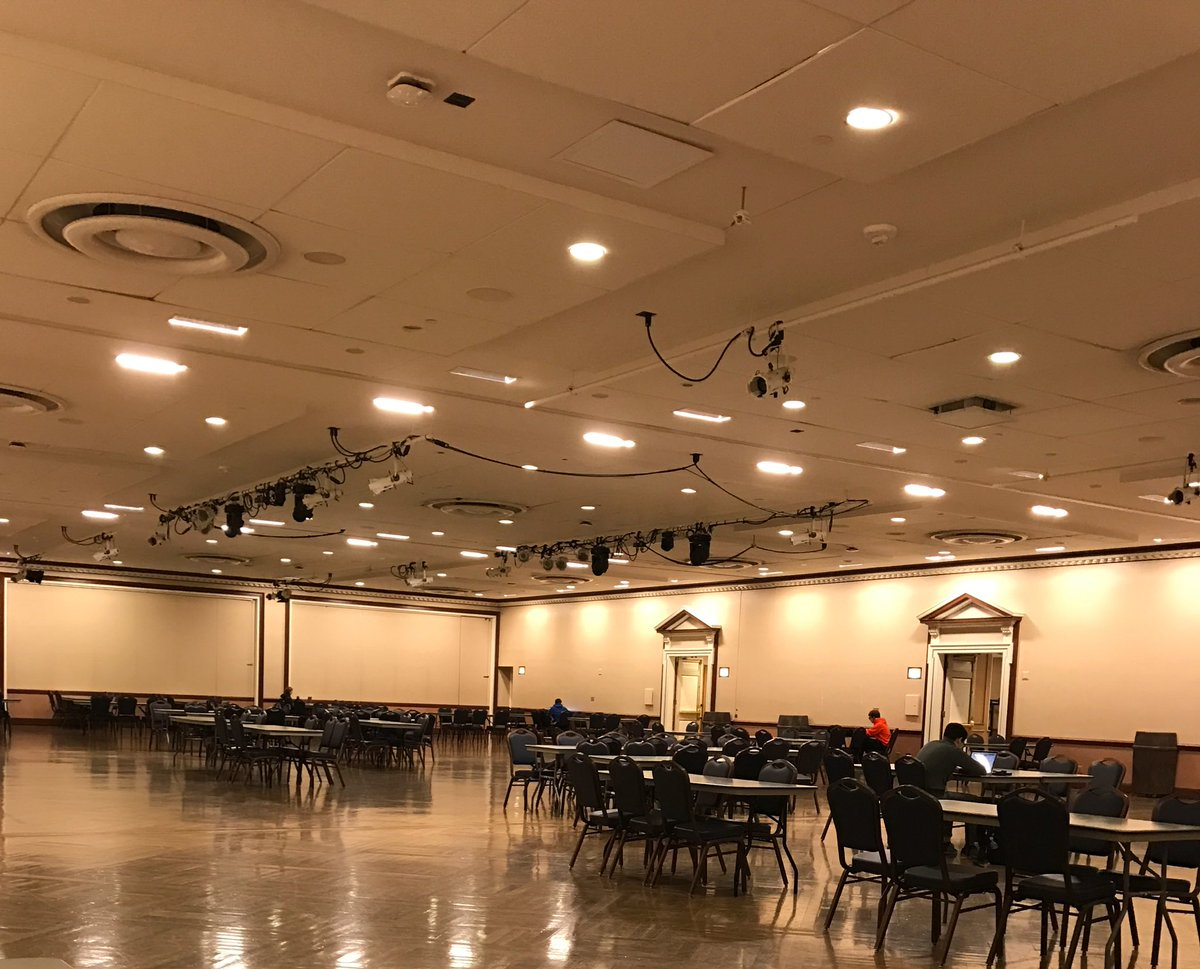
\includegraphics[width=\textwidth]{illinirooms.jpg}
    \caption{The combined Illini rooms with capacity for 496 in round tables.}
\end{figure}


\subsection{Conference Contingency Plan}
In the event that the Union has reduced availability during the conference we have the ability to host technical sessions and workshops at a combination of buildings: The National Center for Supercomputing Applications (NCSA) and Beckman Institute. Rooms in Beckman Institute range from 20 - 60 classroom capacity. Most rooms have A/V capabilities. NCSA has rooms that can hold 13 - 50 people in lecture style. As these buildings are UIUC property, the cost of renting them are significantly reduced compared to a private facility. Additionally, these two buildings are adjacent to one another and are at most a 10 minute walk from the Union. We could also host all technical sessions at the I Hotel. Hosting at the I Hotel is more expensive than hosting in University buildings and would also require additional transportation options. We would need to reevaluate some parts of our budget in order to host the technical program at this venue. See Appendix E on page \pageref{appendix:map} for a map marking the locations of the proposed conference facilities.\\


\textbf{National Center for Supercomputing Applications (NCSA)}\\
NCSA is a hub of transdisciplinary research and digital scholarship where University of Illinois faculty, staff, and students, and collaborators from around the globe, unite to address research grand challenges for the benefit of science and society.\\
\begin{figure}[H]
	\centering
	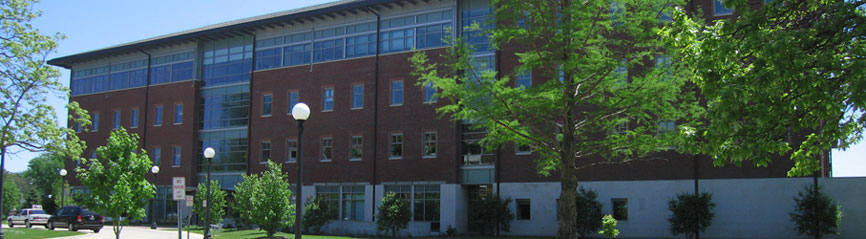
\includegraphics[width=0.8\textwidth]{ncsa_front.jpg}
	\caption{NCSA}
	\label{fig:ncsa}
\end{figure}

\textbf{Beckman Institute}\\
The Beckman Institute for Advanced Science and Technology at the University of Illinois is an interdisciplinary research institute devoted to leading-edge research in the physical sciences, computation, engineering, biology, behavior, cognition, and neuroscience.\\

\begin{figure}[H]
	\centering
	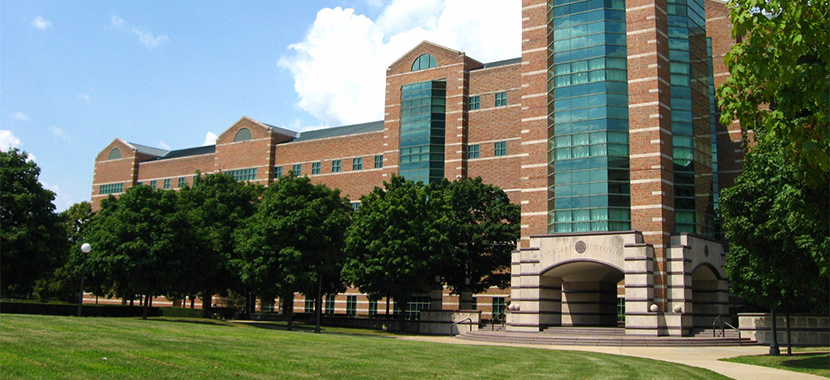
\includegraphics[width=0.8\textwidth]{beckman.jpg}
	\caption{Beckman Institute}
	\label{fig:beckman}
\end{figure}

\textbf{The I Hotel and Conference Center}\\
The IHotel offers a unique, flexible, meeting space and a variety of small touches that make any meeting, social gathering or event in Champaign-Urbana a flawless and memorable experience.\\

\begin{figure}[H]
    \centering
    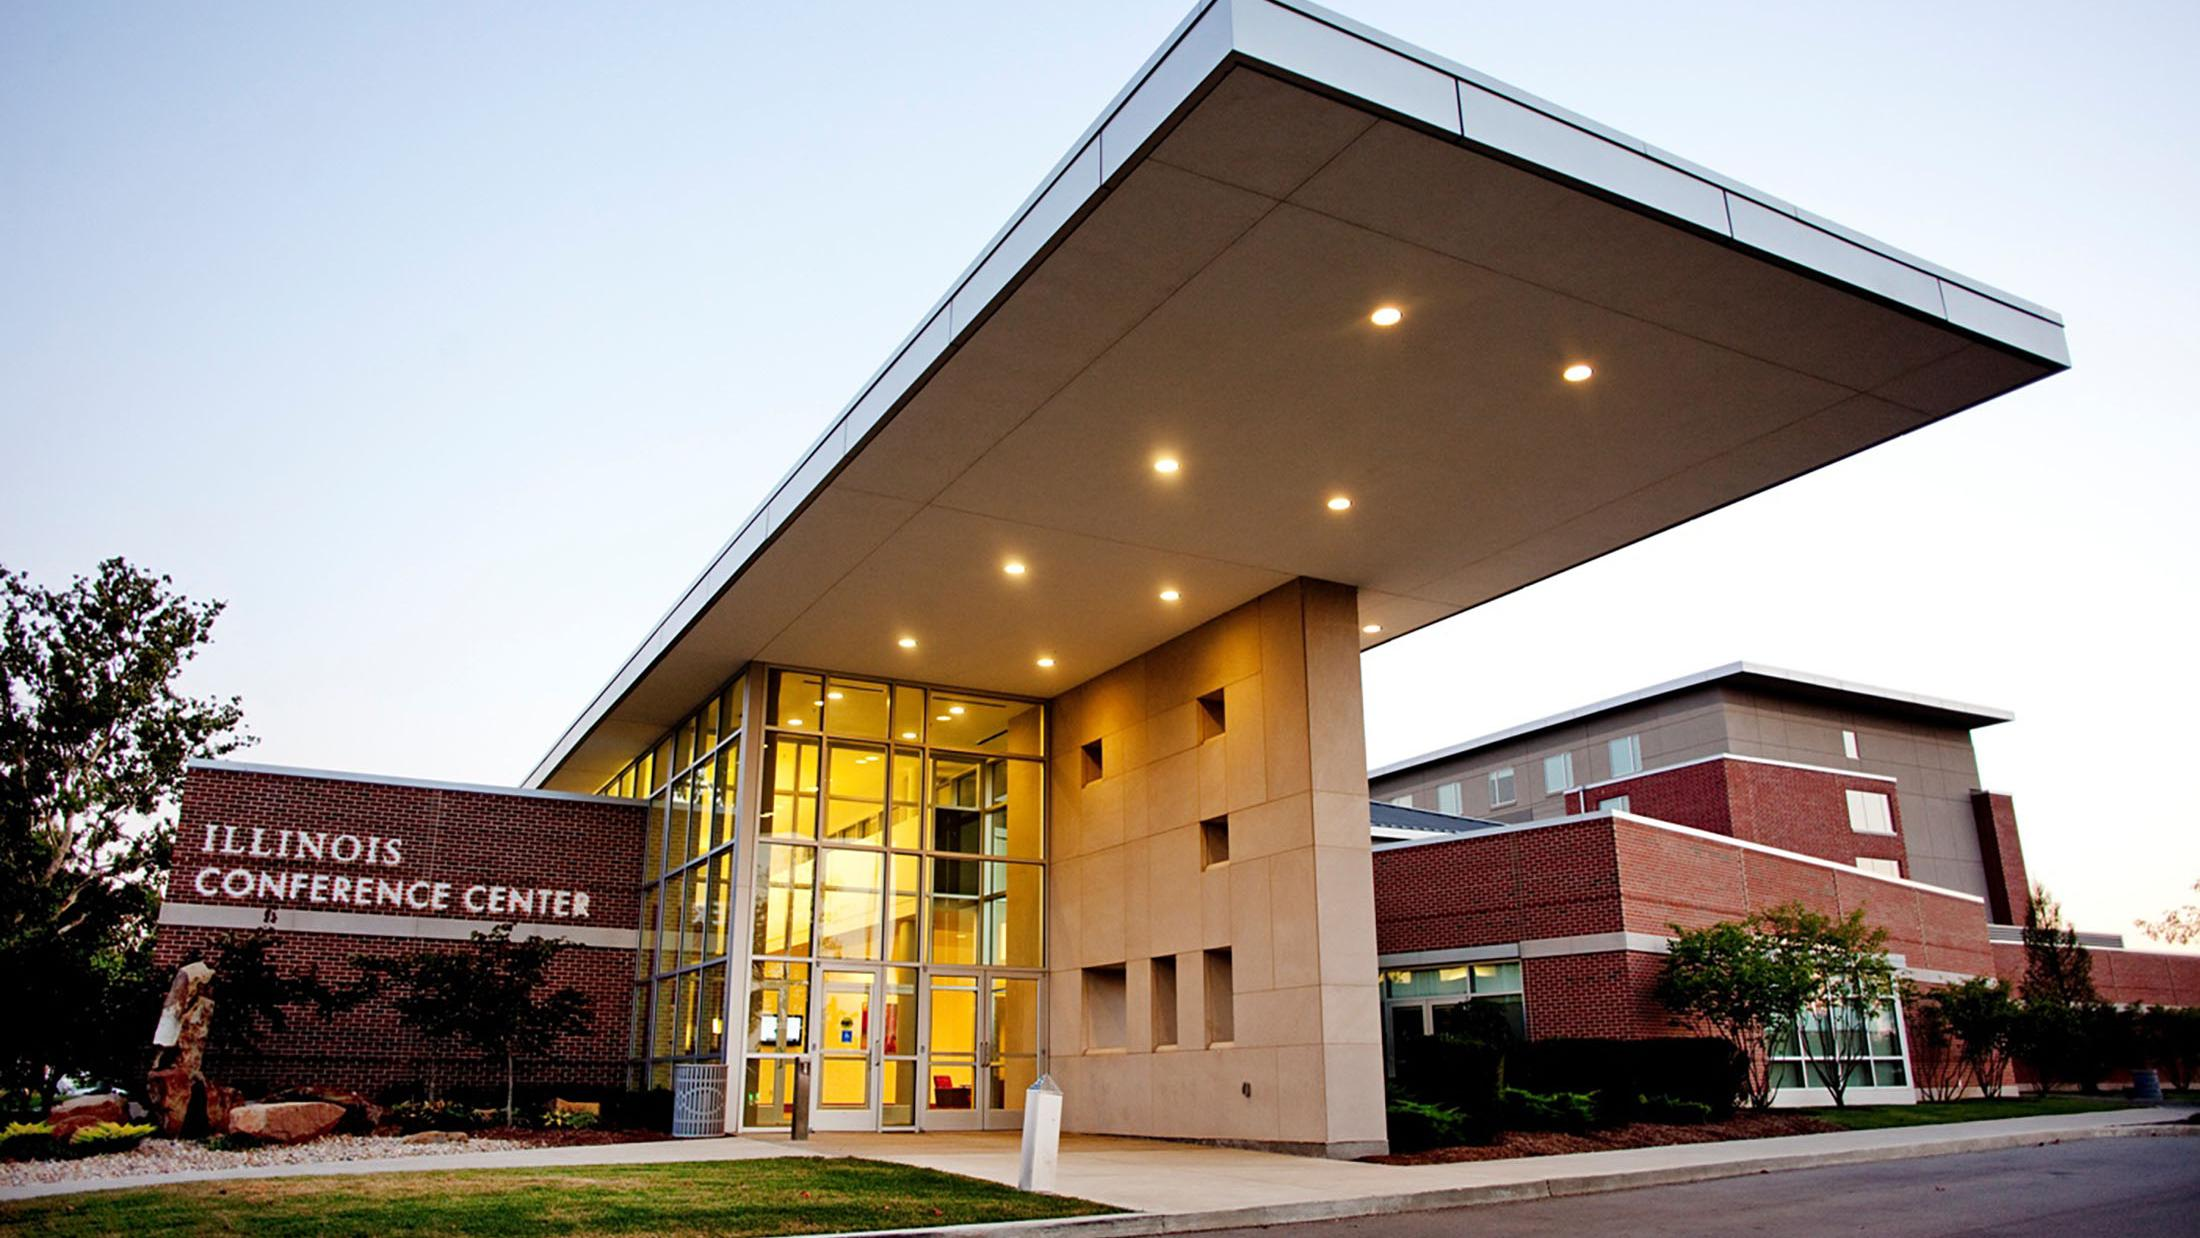
\includegraphics[width=0.8\textwidth]{ihotel.jpg}
    \caption{I Hotel}
    \label{fig:beckman}
\end{figure}

\newpage
\subsection{Hotels and Accommodations}

$\textbf{The Garden Hotel Urbana}$\\
When selecting the primary hotel to accommodate students we considered the ability to host all students under one roof over proximity to the conference activities. The Garden Hotel Urbana (soon to be the Radisson) will be the primary hotel for all attendees. This will also be the location of the opening ceremony dinner. Since this hotel is just beyond walking distance from the main conference activities, we will hire four Peoria Charter busses to shuttle attendees to and from the Union every 10 minutes. Additionally, there is a CU-MTD bus stop adjacent to the hotel that travels directly to the Union and runs every 10 minutes from 8am to 6pm. \\ 
\begin{figure}[H]
	\centering
	\begin{subfigure}{0.5\textwidth}
		\centering
		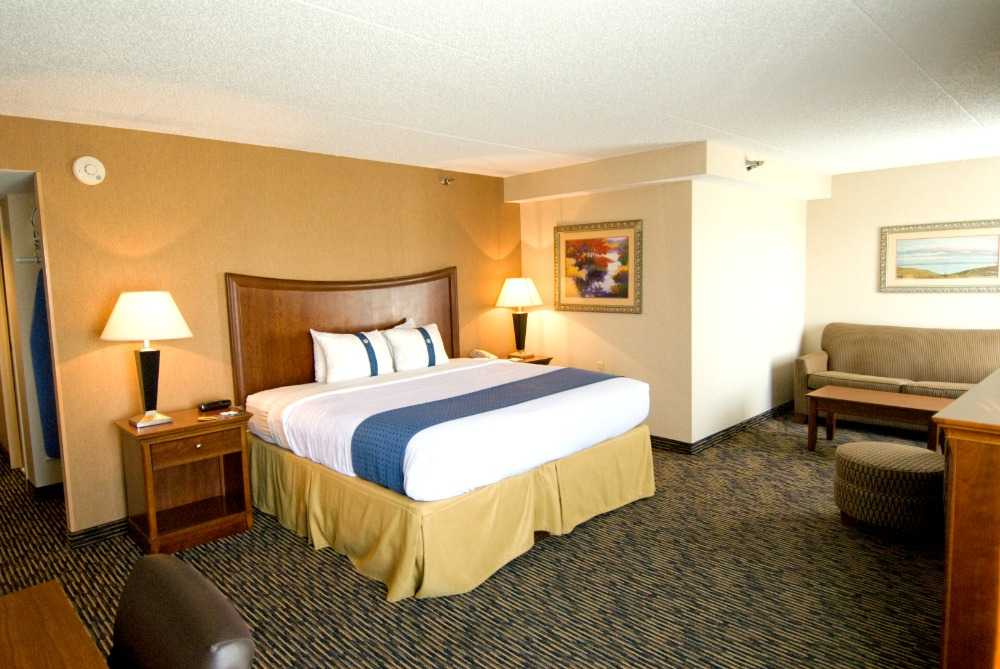
\includegraphics[width=0.9\linewidth]{garden_king.jpg}
		\subcaption{King Suite}
	\end{subfigure}%
	\begin{subfigure}{0.5\textwidth}
		\centering
		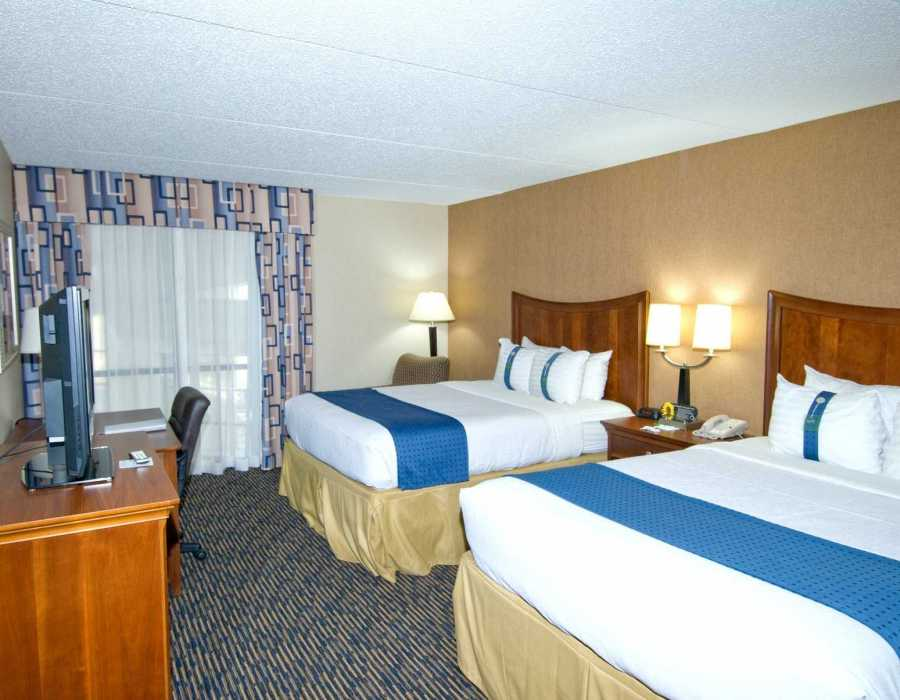
\includegraphics[width=0.9\linewidth]{garden_queen.jpg}
		\subcaption{Queen Double}
	\end{subfigure}
	\caption{Garden Urbana Hotel rooms}		
\end{figure} 

$\textbf{Illini Union}$\\
This is the primary hotel for invited speakers and panelists. Commuting to the conference will be as easy as taking the elevator downstairs because the Illini Union is where the primary conference activities will be held. The Union is also a five-minute walk from Green Street, the campus hub of dining and social activities. Guests have access to Wi-Fi and, upon request, guest passes to the university recreational facilities. Breakfast is provided in the form vouchers for any of the hotel restaurant options inside the Union. Hosting technical sessions, workshops, and plenaries in the Union will help us negotiate a lower room rate.\\

\begin{figure}[H]
	\centering
	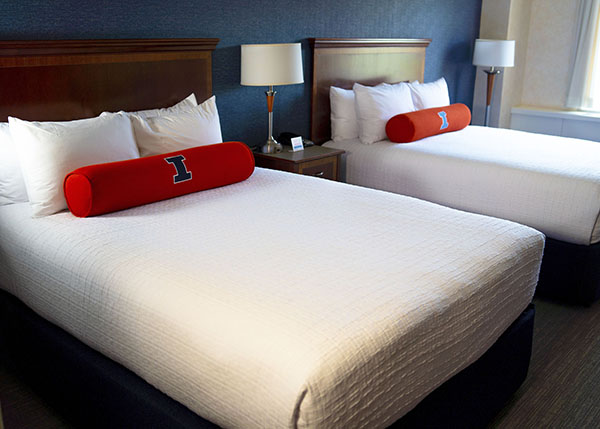
\includegraphics[width=0.5\linewidth]{illini-queen.jpg}
	\caption{Queen Double}		
\end{figure} 

$\textbf{Marriott TowneSuites}$\\
In the event that attendance exceeds 600 people, we will have overflow rooms in the Marriott TowneSuites. Rooms at the Marriott resemble a studio apartment with an open floor plan, refrigerator, stove, microwave,dishes, and dining area. Many rooms are equipped with pull-out couches, allowing 5 students to share a queen double room if desired. The hotel offers internet access for a maximum of 3 devices per room. The hotel is located on Green Street and the Illini Union a mere five-minute walk away. For $\$7$ a day, guests may park in a parking garage with 8ft clearance.\\
\begin{figure}[H]
	\centering
	\begin{subfigure}{0.5\textwidth}
		\centering
		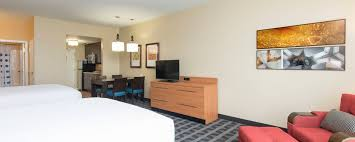
\includegraphics[width=0.9\linewidth]{marriott_room1.jpeg}
	\end{subfigure}%
	\begin{subfigure}{0.5\textwidth}
		\centering
		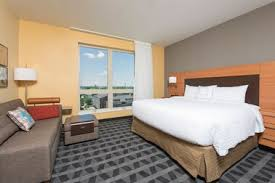
\includegraphics[width=0.9\linewidth]{marriott_room2.jpeg}
	\end{subfigure}
	\caption{Marriott Rooms: Left, a queen double. Right, a king single}		
\end{figure} 

UIUC is one of most well represented schools at past student conferences. Students from UIUC will be able to stay in their respective dorms and apartments to maximize the number of hotel rooms available to out of town guests. 


\begin{table}
\caption{Cost of Hotels}
\label{table:hotels}
	\centering
	\makebox[0.6\linewidth]{\begin{tabular}{lccccc}
	\hline\hline
	\textbf{Hotel} & \textbf{Distance from} & \textbf{Dates} & \textbf{Number of Rooms} & \textbf{Rates*} & \textbf{Per Person**}\\
                & \textbf{the Union (mi)} & & & & \\
	\hline\hline
	Garden Urbana & 2.2  & 4/8-4/11 & 198 & 119 & $\$$29.75\\
	Illini Union & 0.0 & 4/8-4/11 & 35 & 134 & $\$$33.5\\
	Marriott TowneSuites &0.25 & 4/8-4/11 & 95 & 189 & \$47.50\\ 
	\hline
	\end{tabular}}
\subcaption*{\textbf{*}\textit{Price for a queen double}\\ \textbf{**}\textit{Assumes 4 people per room}}
\end{table}

\subsection{Dining}
\subsubsection{Breakfast}
Our primary hotel, the Garden Hotel in Urbana, soon to be the Radisson Hotel, serves complimentary breakfast every morning. Due to this, we will not be catering breakfast at the Illini Union during the conference. Guests staying at the Illini Union Hotel are provided with vouchers for breakfast at the food court in the basement of the Union. The food court offers Einstein Bros, Starbucks, Garbanzo Mediterranean, and more. 
\subsubsection{Lunch}
Conference attendees are encouraged to explore the University’s campus and surroundings, including getting lunch on the main street of campus, Green street. Due to this, lunch will not be provided for the conference. However, box lunches will be provided for the Student Sections Committee meeting from 11:30pm to 1:30pm on Friday as well as any lunch and learns hosted by sponsors on Friday and Saturday. The Illini Union’s catering service, University Catering, will be used. Sponsors can also choose to sponsor and host a lunch in one of the technical session rooms on Friday or Saturday. If more rooms are required, there are available rooms on the first and second floor of the Union. Sponsors will be able to use University Catering, or cater from one of the food vendors in the Illini Union.
\subsubsection{Dinner}

\textbf{Thursday Night}\\
Communicating the science of nuclear energy remains one of the chief challenges of our field. The opening dinner of this conference will focus on science communication and the people behind the science. Science communication requires more than the recitation of raw data to be effective. By telling our own, diverse backstories, we become more effective science communicators. Speakers will be asked to speak to their own backstory as a nuclear advocate and how their story makes them a more effective communicator.\\\\
\indent\textbf{Friday Night}\\
The second dinner will be themed around networking and professional-development and how these critical tools have value beyond finding jobs. Communities like ANS thrive on the exchange of ideas and knowledge. The student conference serves plays an essential role by connecting the burgeoning minds of the next generation with the wisdom of established professionals. This dinner will consist of tables organized by company/national lab to allow students and professionals to mingle, promoting the exchange of ideas.\\\\ 
\indent\textbf{Saturday Night}\\
The closing dinner of the conference will be a call to action for student attendees. Ours is a generation faced with challenges on a scale never witnessed by humanity, and we will only successfully address these challenges through the engagement of as many bright young minds as possible. The speakers for this night will be asked to address ways we all can take individual responsibility for the grand challenges of our age by using our own unique skills to tackle problems like climate change and energy poverty from every angle imaginable.\\ 
\subsection{Travel and Transportation}

\subsubsection{Getting to Champaign}
The University of Illinois is a 2.5 hour drive from one of the largest airports in the world, O'Hare International Airport. There is also a small airport located just 20 minutes outside of campus. Additionally, there is a reliable bus service, Peoria Charter, that runs between O'Hare and the UIUC campus several times per day. Table \ref{table:airfare} shows the round-trip, non-stop, airfare costs for the first weekend of April. Peoria Charter fare from O'Hare to UIUC is currently $\$61$ round-trip. Due to the central location of UIUC, driving might be a good option for some schools and individuals. Table \ref{table:ground} shows the approximate driving times and costs from several universities. 

\begin{table}[H]
\caption{Estimated Costs of Ground Travel}
\label{table:ground}
   \begin{tabular}{lcccc}
   \hline\hline
   \textbf{School}&\textbf{Estimated Mileage (mi)}&\textbf{Driving Time (hrs)}&\textbf{Fuel Cost*}&\textbf{Per Person**}\\
   \hline\hline
    Purdue University&90&1h 40m&\$21.86&\$5.47\\
    University of Cincinnati&233& 3h 40m&\$56.60&\$14.15\\
    Air Force Tech &250&3h 58m&\$60.73&\$15.18\\
    University of Wisconsin&253&4h&\$61.46&\$15.36\\
    Missouri University S \& T &279&4h 21m&\$67.77&\$16.94\\
    U. Missouri - Columbia&291&4h 28m&\$70.69&\$17.67\\
    Ohio State University&302&4h 47m&\$73.36&\$18.34\\
    University of Michigan&345&5h 17m&\$83.81&\$20.95\\
    Vanderbilt University&373&5h 33m&\$90.61&\$22.65\\
    Iowa State University&378&5h 44m&\$91.82&\$22.96\\
    \hline
    Average&279&4h 22m&\$67.87&\$16.97

    \end{tabular} 
\end{table}
\noindent\textbf{*}\textit{Estimated assuming an average 23 MPG}\\
\textbf{**}\textit{Assumes four people in a car}

\subsubsection{Getting to the Conference}
The primary hotel, Garden Hotel Urbana, is approximately two miles from the Union and outside of reasonable walking distance. Thus we have budgeted to include transportation provided by Peoria Charter. We intend to have busses shuttling continuously between the Union and the Garden Hotel Urbana. For those who desire more flexibility and freedom, there is CU-MTD bus stop adjacent to the hotel that has a bus every 10 minutes. This bus route, the 22 Illini, can take attendees directly to the Union from the hotel. It is also one of the main campus bus routes and can take travelers almost anywhere on or around campus. Lyft and Uber are available as well for attendees that choose to use those services. A map of the bus route is in Appendix E: Campus Map of Locations on page \pageref{appendix:map}.

\begin{table}[H]
\caption{Airfare to Chicago/Champaign}
\label{table:airfare}
   \begin{tabular}{lccc}
   	\hline\hline
    \textbf{School} & \textbf{Departure City} & \textbf{O'Hare (ORD)*} & \textbf{Willard (CMI)} \\
    \hline\hline
    University of California - Berkeley & San Francisco (SFO) & $\$$338 & $\$$436 \\
    University of California - Irvine&Orange County (SNA)&$\$$394&$\$$436\\
    Colorado School of Mines & Denver (DEN) & $\$$222 & $\$$328 \\
    Three Rivers Community College & Hartford (BDL) & $\$$468 & $\$$327 \\ 
    University of Florida & Gainesville (GNV)& $\$$377 & $\$$416 \\
    Georgia Institute of Technology & Atlanta (ATL)& $\$$199 & $\$$291 \\
    Southern Polytechnic State University & Atlanta (ATL) & $\$$199 & $\$$291 \\
    Idaho State University & Idaho Falls (IDA) & $\$$501 & NA \\
    Kansas State University & Manhattan (MHK) & $\$$336 & $\$$406 \\ 
    Louisiana State University & Baton Rouge (BTR) & $\$$380 & $\$$329 \\
    United States Naval Academy & Hanover (BWI) & $\$$210 & $\$$321 \\  
    University of Maryland & Hanover (BWI)&$\$$210 &$\$$321 \\ 
    Massachusetts Institute of Technology & Boston (BOS)&$\$$191 &$\$$325 \\ 
    University of Massachusetts - Lowell &Boston (BOS) &$\$$191 &$\$$325 \\
    University of Nevada - Las Vegas & Las Vegas (LAS)& $\$$262 &$\$$358 \\ 
    University of New Mexico &Albuquerque (ABQ) &$\$$439 &$\$$358 \\ 
    City College of New York &\$New York (JFK) &$\$$245 &$\$$325 \\
    Excelsior College & Albany (ALB) &$\$$444 &$\$$327 \\ 
    Rensselaer Polytechnic Institute & Albany (ALB)&$\$$444 &$\$$327 \\ 
    United States Military Academy at West Point&New Windsor (SWF)&$\$$273 &$\$$357 \\ 
    North Carolina State University &Morrisville (RDU) &$\$$180 &$\$$321 \\
    Oregon State University &Portland (PDX) &$\$$314 &$\$$436 \\ 
    Pennsylvania State University & Harrisburg (MDT)&$\$$397 & $\$$323 \\
    University of Pittsburgh &Pittsburgh (PIT) &$\$$282 &$\$$293 \\ 
    Clemson University&Greenville (GSP)&$\$$356&$\$$287\\
    South Carolina State University&Columbia (CAE)&$\$$407 &$\$$564 \\ 
    University of South Carolina&Columbia (CAE)&$\$$407&$\$$564\\
    Chattanooga State Comunity College&Chattanooga (CHA)&$\$$334&$\$$316\\
    University of Tennessee&Knoxville (TYS)&$\$$340&$\$$291\\
    Texas A\&M University&College Station (CLL)&$\$$367&$\$$243\\
    University of Texas - Arlington&Dallas (DFW)&$\$$197&$\$$303\\
    University of Texas - Austin&Austin (AUS)&$\$$298&$\$$358\\
    University of Texas - Permian Basin&Midland (MAF)&$\$$434&$\$$333\\
    Utah State University&Salt Lake City (SLC)&$\$$298&$\$$358\\
    University of Utah&Salt Lake City (SLC)&$\$$298&$\$$358\\
    Virginia Commonwealth University&Richmond (RIC)&$\$$279&$\$$321\\
    University of Washington&Seattle (SEA)&$\$$253&$\$$436\\
    \hline
    Average Lowest Cost for Air Travel**&$\$$293&&
    \end{tabular} 
\end{table}

\noindent\textbf{*}\textit{A \$61 round-trip bus ticket through Peoria Charter was added to the cost.}\\
\textbf{**}\textit{The average of the lowest price between O'Hare and Willard.}\\


